\section{Various Exoplanet Spectra}

Figure~\ref{fig:earth} shows the spectrum of Earth. In the case of Earth, the atmosphere is relatively thin, so the thermal emission is close to a blackbody spectrum at the radiative equilibrium temperature. The reflection spectrum, on the other hand, corresponds to the stellar spectrum modulated by atmospheric absorption.  

Figure~\ref{fig:bd} shows the spectrum of a brown dwarf. It deviates significantly from a pure blackbody spectrum.  

Figure~\ref{fig:jwst} presents the JWST/NIRSpec spectrum of the hot Saturn WASP-39b, where prominent molecular absorption features are clearly visible.  

\begin{figure}[]
\begin{center}
	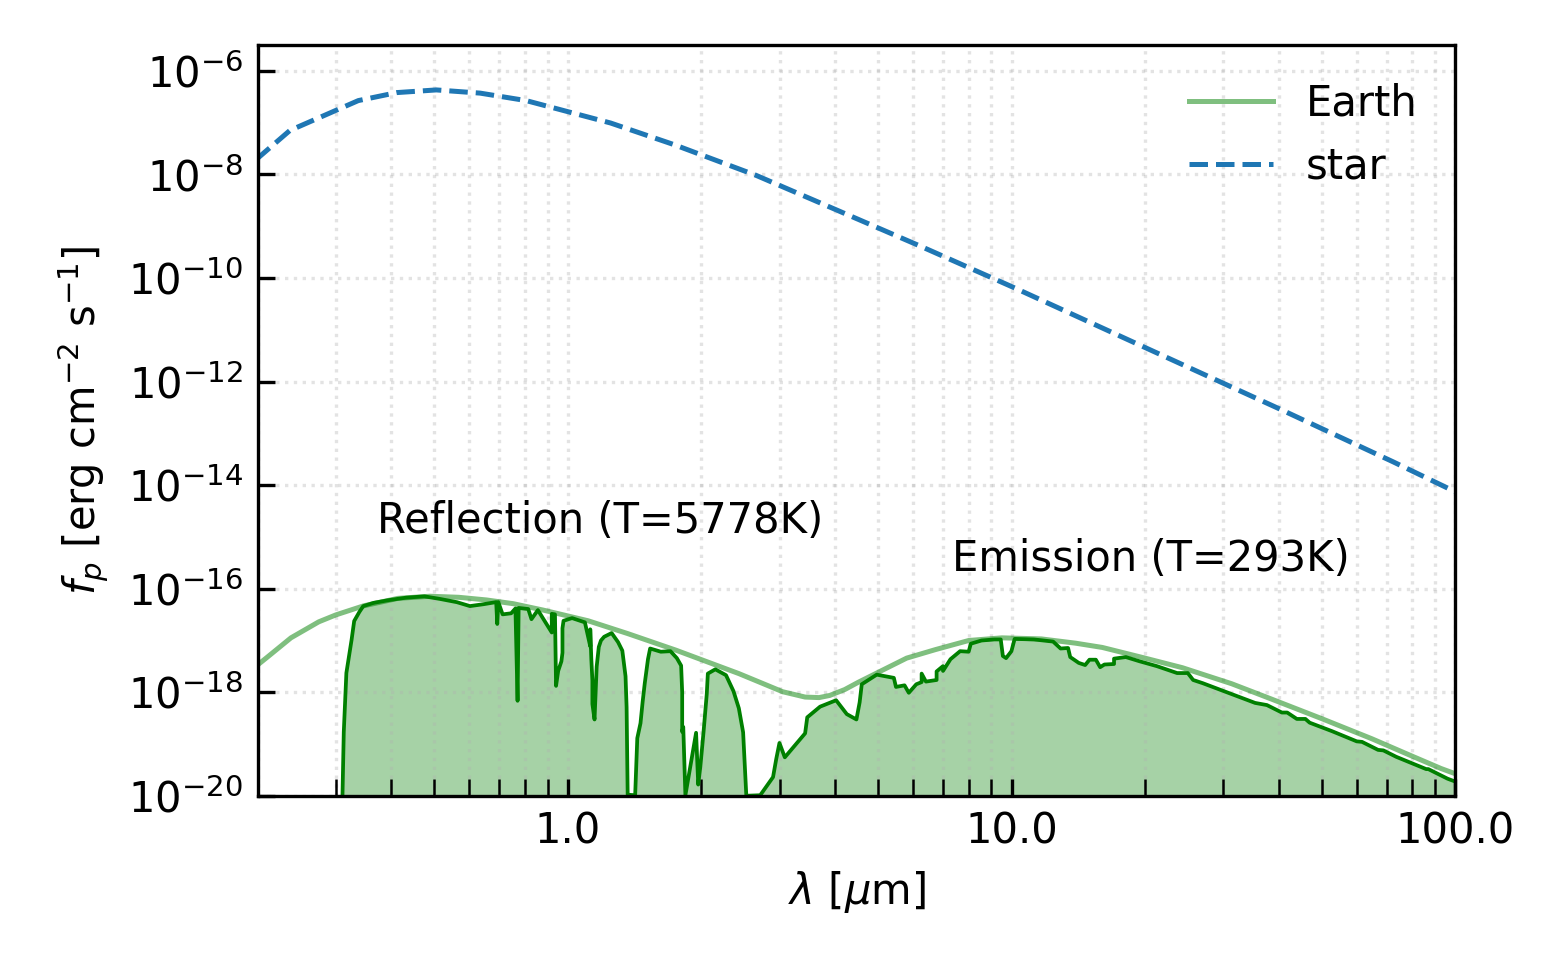
\includegraphics[width=\linewidth]{fig/EarthEmis.png}
\end{center}
\caption{Spectrum and contrast of Earth.}
\label{fig:earth}
\end{figure}

\begin{figure}[]
\begin{center}
	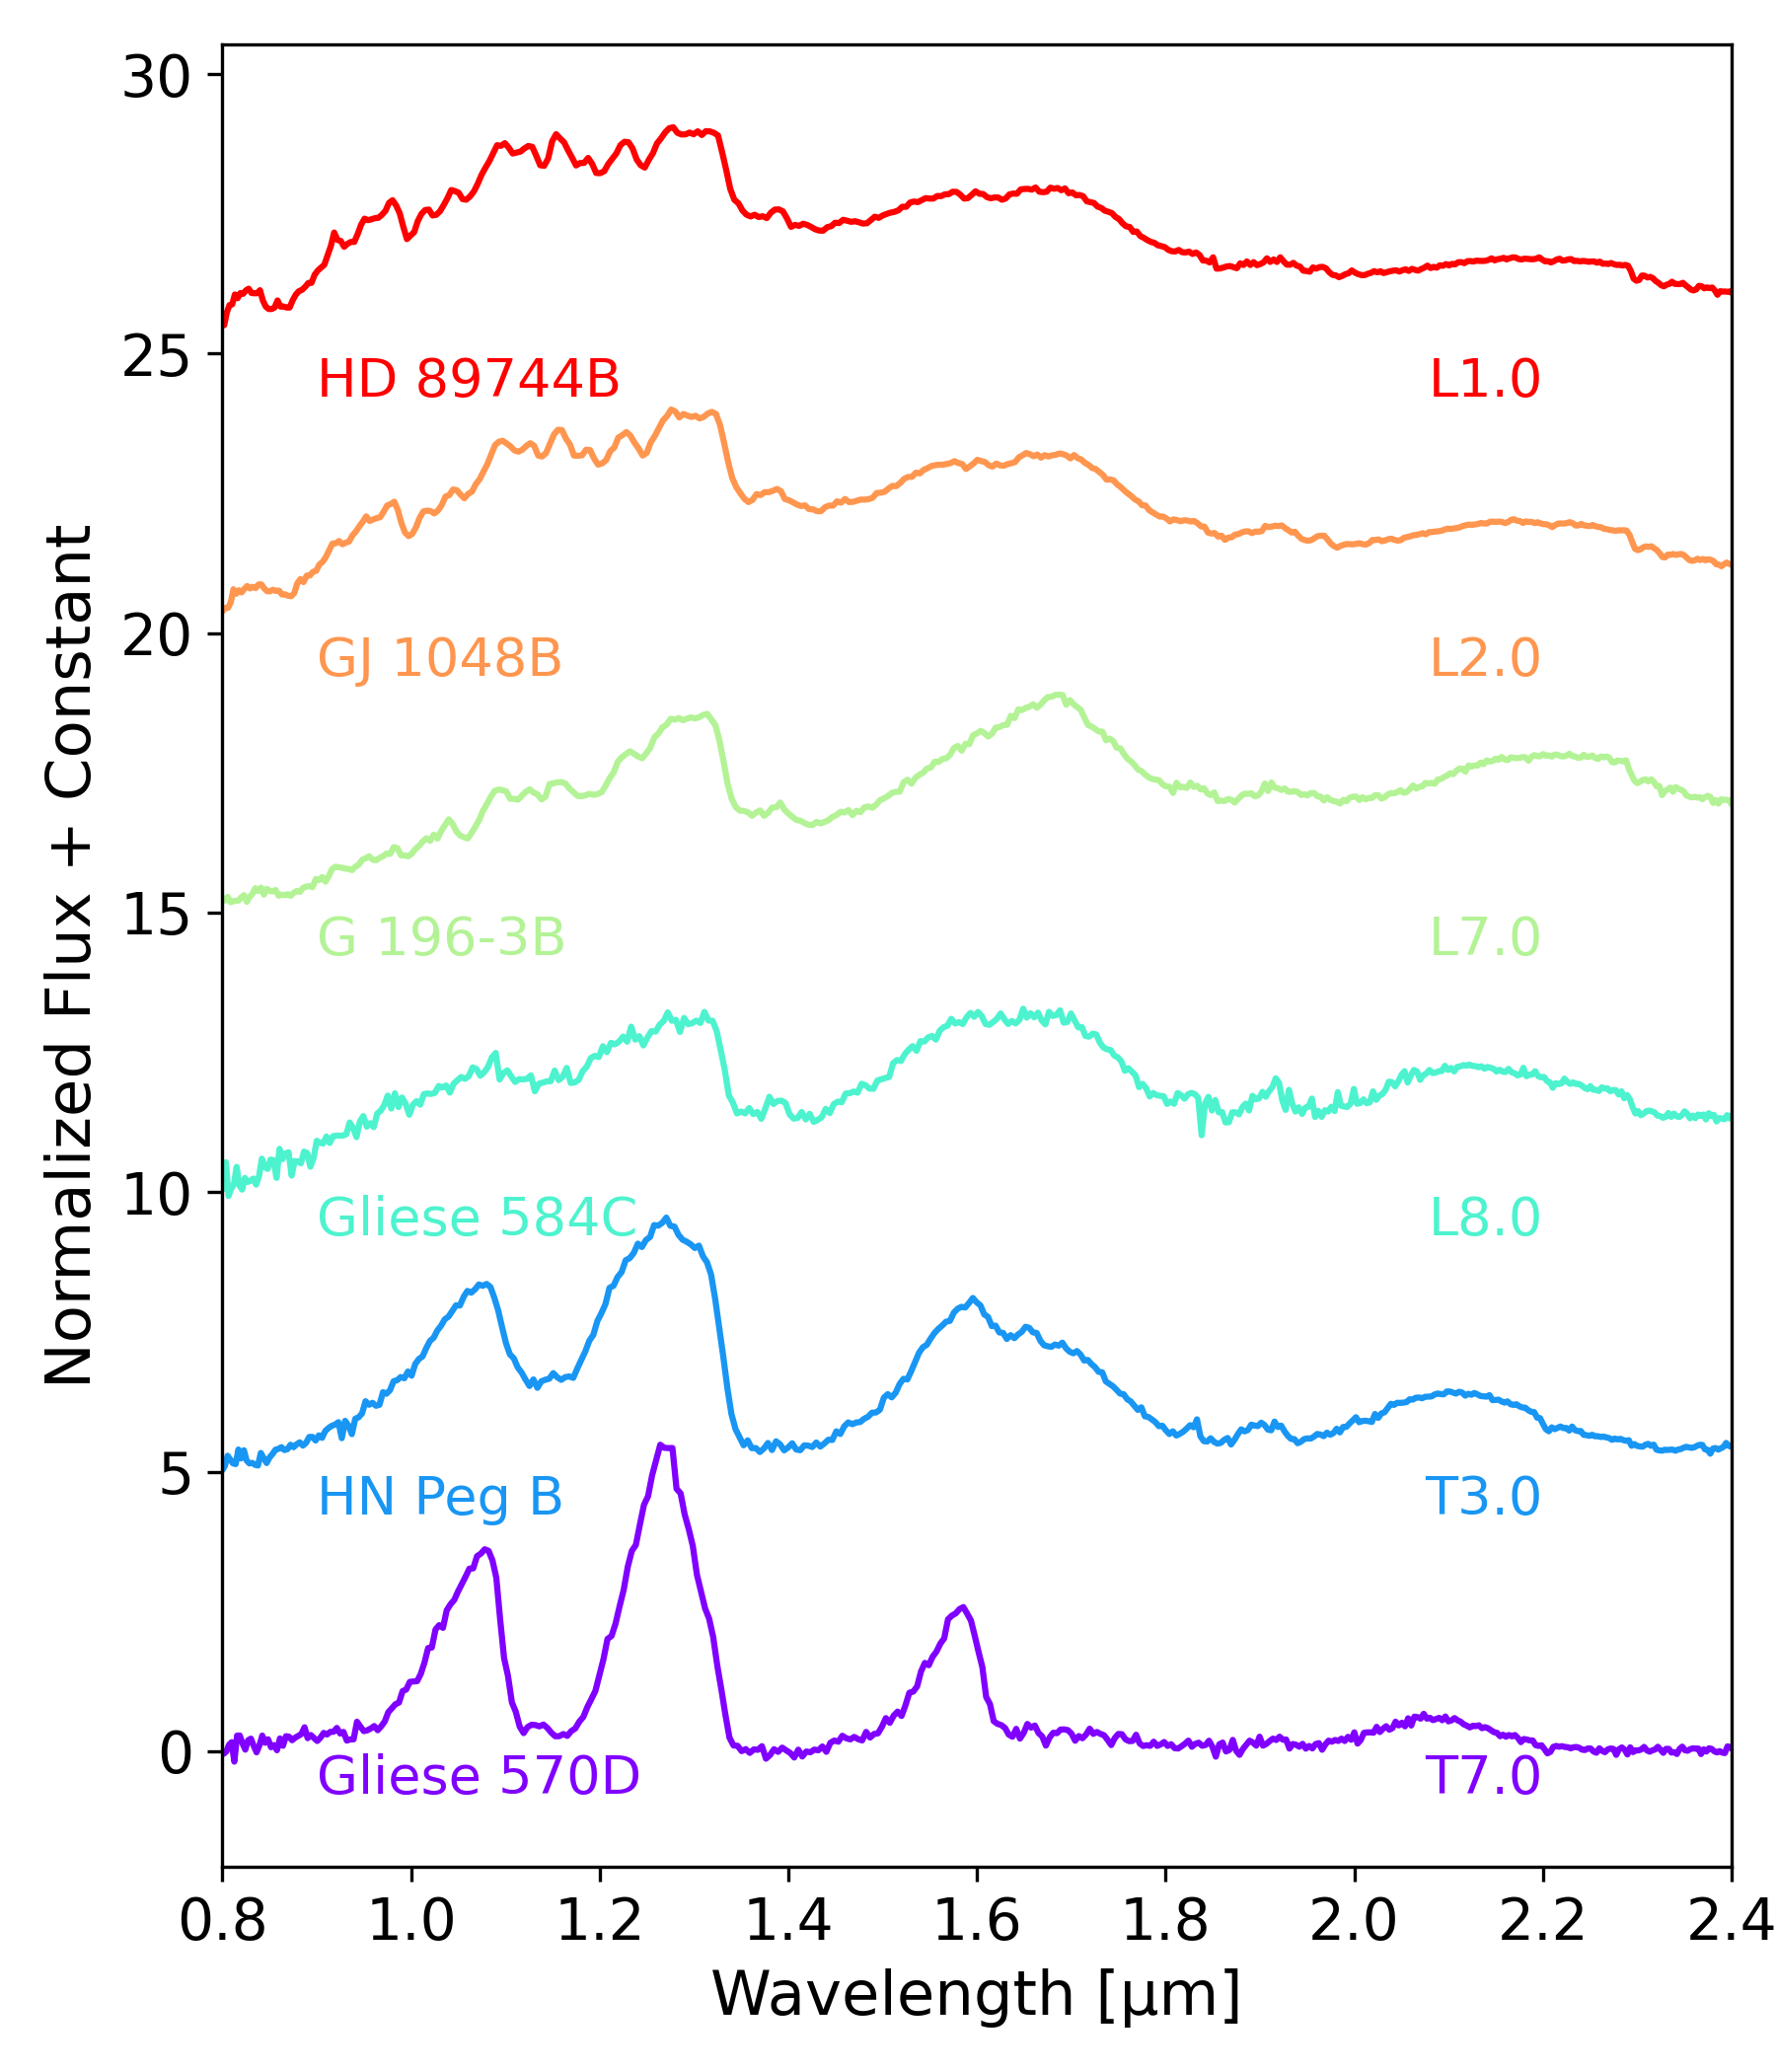
\includegraphics[width=\linewidth]{fig/bdspectra.png}
\end{center}
\caption{Spectrum of a brown dwarf, from SpeX Prism library.  Inspired by \cite{2025ApJ...988...31L}.}
\label{fig:bd}
\end{figure}

\begin{figure*}[htb]
\begin{center}
	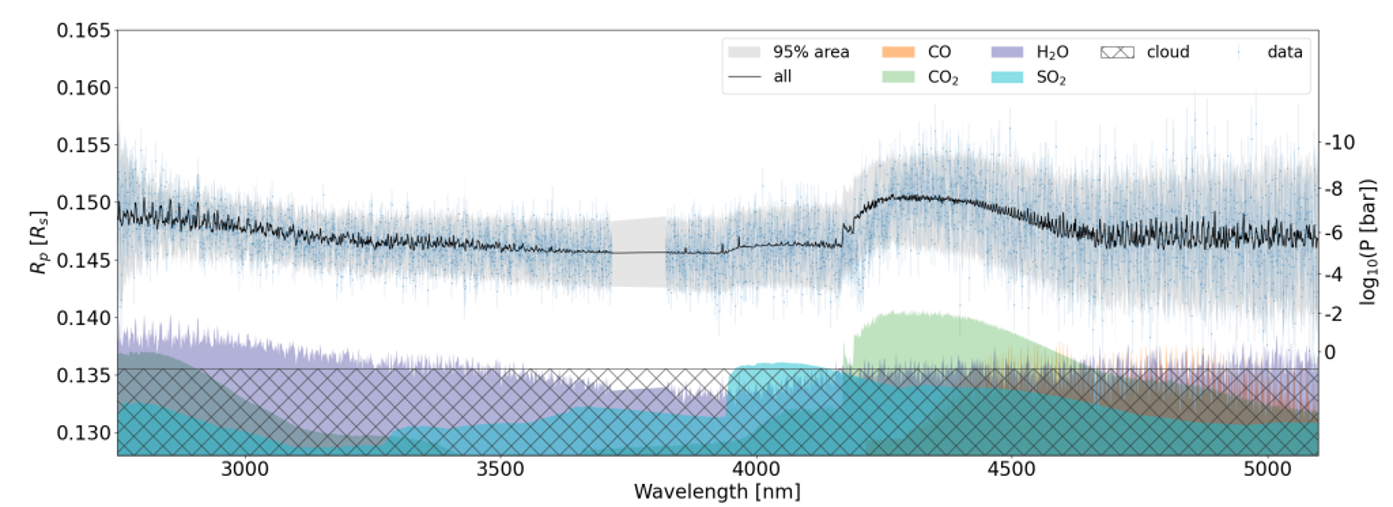
\includegraphics[width=\linewidth]{fig/jwst_spectrum.png}
\end{center}
\caption{JWST transmission spectrum of WASP-39b \cite{2025ApJ...985..263K}.}
\label{fig:jwst}
\end{figure*}

